\section{Architettura Back-End} \label{sec:archback}

Coerentemente alla struttura imposta dall'adozione di una Clean Architecture, il back-end dell'applicazione è organizzato tramite delle classi controller, use case, repository e data source.\\
Per collegare l'interfaccia grafica lato front-end con il funzionamento dell'applicativo lato back-end, sono state implementate delle server actions per chiamare i controller relativi all'azione desiderata.\\
I controller eseguono la chiamata allo use case relativo, che costituisce ed implementa la business logic dell'intero sistema.\\
Per accedere alle fonti dei dati, necessari a realizzare le funzionalità definite dai casi d'uso, le classi use cases si relazionano con delle classi repositories, nelle quali è posta la logica di persistenza, che presentano i metodi per lettura, scrittura ed eliminazione dei dati.\\
La singola classe repository si interfaccia alla classe data source ad essa associata, la quale presenta i metodi che intervengono concretamente sulle fonti dei dati per compiere le funzioni richieste sui database.\\
Una volta terminate le operazioni nel data source, il controllo torna alla repository, la quale ritorna i dati recuperati allo use case quando richiesto. Completata la funzionalità definita dal caso d'uso, il flusso di controllo torna al controller che dovrà gestire la risposta verso la server action da cui tutto è iniziato.

\begin{figure}[h!]
    \centering  
    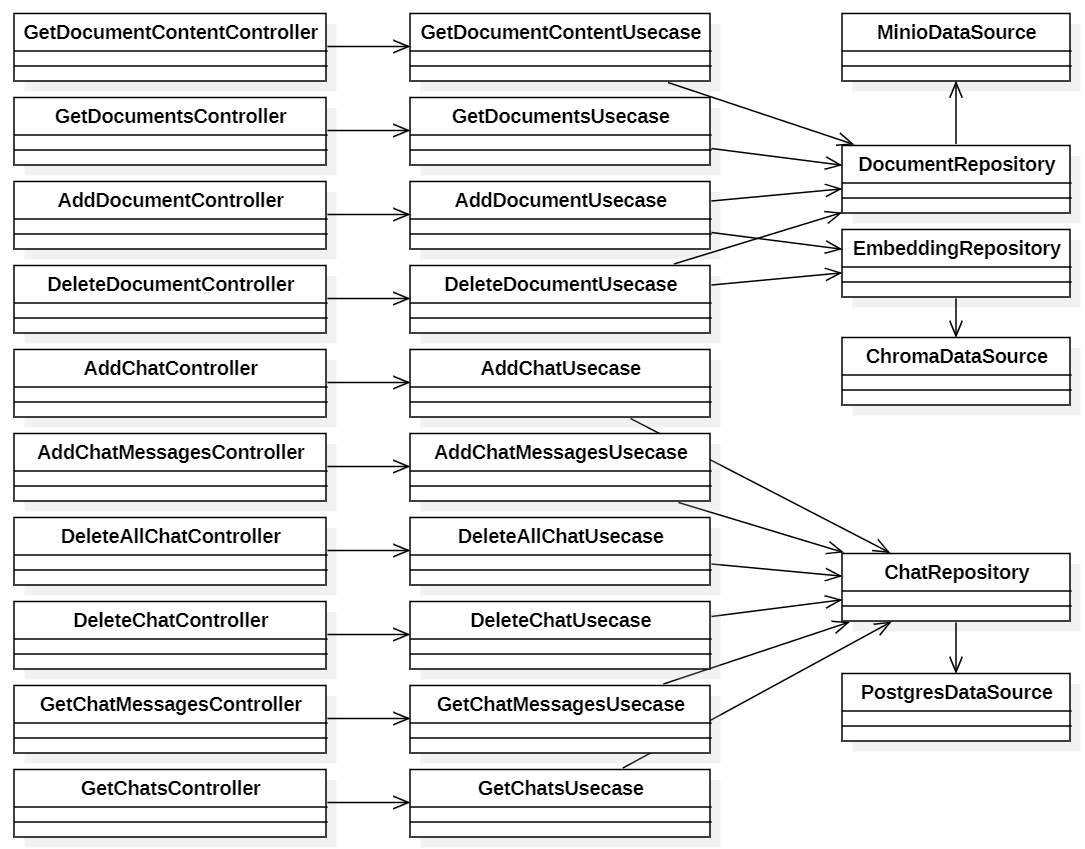
\includegraphics[width=0.95\textwidth]{backendview.png}
    \caption{UML introduttivo delle classi del back-end}
\end{figure}

\newpage


\subsection{Server Actions} \label{subsec:serveractions}

\subsubsection{addDocument}
\textbf{Parametri}
\begin{itemize}
    \item \textit{data: FormData}.
\end{itemize}
\textbf{Descrizione}\\
Questa funzione asincrona lato server effettua una chiamata a AddDocumentController, passando il parametro data. Data contiene una \textit{string} model e un \textit{File} file, che rappresentano il modello che deve presentare il nuovo documento e il file da aggiungere. Gestisce l'aggiunta di un documento inviando i dati al controller e si occupa di gestire eventuali errori che si possono verificare durante il processo.


\subsubsection{deleteDocument}
\textbf{Parametri}
\begin{itemize}[itemsep=-4pt]
    \item \textit{name: string};
    \item \textit{model: IModel}.
\end{itemize}
\textbf{Descrizione}\\
Questa funzione asincrona lato server effettua una chiamata a DeleteDocumentController, passando i parametri name e model, che rappresentano il nome del documento da eliminare e il modello che non deve più presentare tale documento. Gestisce l'eliminazione di un documento inviando i dati al controller e si occupa di gestire eventuali errori che si possono verificare durante il processo.

\subsubsection{getDocument}
\textbf{Parametri}
\begin{itemize}
    \item \textit{model: IModel}.
\end{itemize}
\textbf{Descrizione}\\
Questa funzione asincrona lato server effettua una chiamata a GetDocumentsController, passando il parametro model, che rappresenta il modello da cui prendere i documenti associati. Gestisce il recupero delle informazioni dei documenti inviando i dati al controller e si occupa di gestire eventuali errori che si possono verificare durante il processo.

\subsubsection{getDocumentContent}
\textbf{Parametri}
\begin{itemize}[itemsep=-4pt]
    \item \textit{docName: string};
    \item \textit{model: IModel}.
\end{itemize}
\textbf{Descrizione}\\
Questa funzione asincrona lato server effettua una chiamata a GetDocumentContentController, passando i parametri docName e model, che rappresentano il nome del documento da cui recuperare il link per la visualizzazione e il modello che presenta tale documento. Gestisce il recupero dell'informazione inviando i dati al controller e si occupa di gestire eventuali errori che si possono verificare durante il processo.

\subsubsection{updateDocument}
\textbf{Parametri}
\begin{itemize}[itemsep=-4pt]
    \item \textit{docName: string};
    \item \textit{model: IModel};
    \item \textit{updatedMetadas: Metadatas}.
\end{itemize}
\textbf{Descrizione}\\
Questa funzione asincrona lato server effettua una chiamata a UpdateDocumentController, passando i parametri docName, model e updatedMetadas, che rappresentano il nome del documento da aggiornare, il modello che presenta tale documento e il nuovo valore che deve avere il tag di visibilità del documento. Gestisce la modifica delle informazioni inviando i dati al controller e si occupa di gestire eventuali errori che si possono verificare durante il processo.

\subsubsection{addChat}
\textbf{Parametri}
\begin{itemize}
    \item \textit{title: string}.
\end{itemize}
\textbf{Descrizione}\\
Questa funzione asincrona lato server effettua una chiamata a AddChatController, passando il parametro title, che rappresenta il nome della sessione di conversazione da aggiungere. Gestisce la creazione della sessione inviando i dati al controller e si occupa di gestire eventuali errori che si possono verificare durante il processo.

\subsubsection{addChatMessages}
\textbf{Parametri}
\begin{itemize}
    \item \textit{messages: ICustomMessages}.
\end{itemize}
\textbf{Descrizione}\\
Questa funzione asincrona lato server effettua una chiamata a AddChatMessagesController, passando il parametro messages, che rappresenta il messaggio da salvare relativo ad una sessione di conversazione. Gestisce il salvataggio del messaggio inviando il dato al controller e si occupa di gestire eventuali errori che si possono verificare durante il processo.

\subsubsection{deleteAllChat}
\textbf{Descrizione}\\
Questa funzione asincrona lato server effettua una chiamata a DeleteAllChatController per eliminare tutti i dati relativi a sessioni e chat history. Gestisce l'eliminazione di queste informazioni effettuando una chiamata al controller e si occupa di gestire eventuali errori che si possono verificare durante il processo.

\subsubsection{deleteChat}
\textbf{Parametri}
\begin{itemize}
    \item \textit{id: number}.
\end{itemize}
\textbf{Descrizione}\\
Questa funzione asincrona lato server effettua una chiamata a DeleteChatController, passando il parametro id, che rappresenta il valore univoco della sessione di conversazione da eliminare. Gestisce l'eliminazione della sessione inviando i dati al controller e si occupa di gestire eventuali errori che si possono verificare durante il processo.

\subsubsection{getChatMessages}
\textbf{Parametri}
\begin{itemize}
    \item \textit{id: number}.
\end{itemize}
\textbf{Descrizione}\\
Questa funzione asincrona lato server effettua una chiamata a GetChatMessagesController, passando il parametro id, che rappresenta il valore univoco della sessione di conversazione da cui recuperare la chat history. Gestisce il recupero dati della sessione inviando il parametro al controller e si occupa di gestire eventuali errori che si possono verificare durante il processo.

\subsubsection{getChats}
\textbf{Descrizione}\\
Questa funzione asincrona lato server effettua una chiamata a GetChatsController, con cui recupera le informazioni delle sessioni di conversazione attive nell'applicazione. Gestisce il recupero dati delle sessioni ed eventuali errori che si possono verificare durante il processo.

\newpage

\subsection{Controllers} \label{subsec:controllers}
\subsubsection{AddDocumentController}
\textbf{Decoratori}
\begin{itemize}
    \item \textit{@injectable()}: decoratore per la Dependency Injection mediante Tsyringe.
\end{itemize}
\textbf{Attributi}
\begin{itemize}
    \item private readonly \textit{\_useCase: AddDocumentUsecase}.
\end{itemize}
\textbf{Metodi}
\begin{itemize}
    \item \textit{handle(data: FormData): Promise<Response>}.
\end{itemize}
\textbf{Descrizione}\\
Questa classe controller, chiamata tramite la server action addDocument, gestisce la chiamata al AddDocumentUsecase per aggiungere a sistema un nuovo documento, passando un \textit{FormData} contenente una \textit{string} model e un \textit{File} file, che rappresentano il modello che deve presentare il nuovo documento e il file da aggiungere.\\ \\
\textbf{Dipendenze}
\begin{itemize}
    \item AddDocumentUsecase.
\end{itemize}

\begin{figure}[h!]
    \centering  
    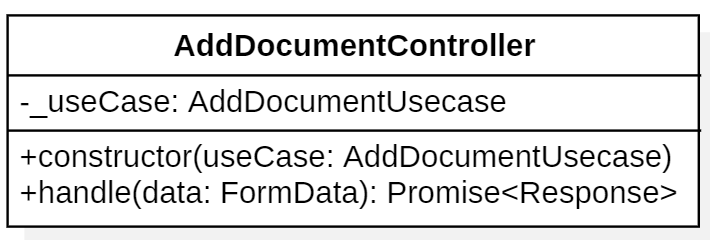
\includegraphics[width=0.5\textwidth]{AddDocumentController.png}
    \caption{UML della classe AddDocumentController}
\end{figure}

\subsubsection{DeleteDocumentController}
\textbf{Decoratori}
\begin{itemize}
    \item \textit{@injectable()}: decoratore per la Dependency Injection mediante Tsyringe.
\end{itemize}
\textbf{Attributi}
\begin{itemize}
    \item private readonly \textit{\_useCase: DeleteDocumentUsecase}.
\end{itemize}
\textbf{Metodi}
\begin{itemize}
    \item \textit{handle(docName: string, model: IModel): Promise<Response>}.
\end{itemize}
\textbf{Descrizione}\\
Questa classe controller, chiamata tramite la server action deleteDocument, gestisce la chiamata al DeleteDocumentUsecase per eliminare dal sistema un documento, passando una \textit{string} docName e una \textit{string} model, che rappresentano il nome del documento da eliminare e il modello da cui rimuoverlo.\\ \\
\textbf{Dipendenze}
\begin{itemize}
    \item DeleteDocumentUsecase.
\end{itemize}

\begin{figure}[h!]
    \centering  
    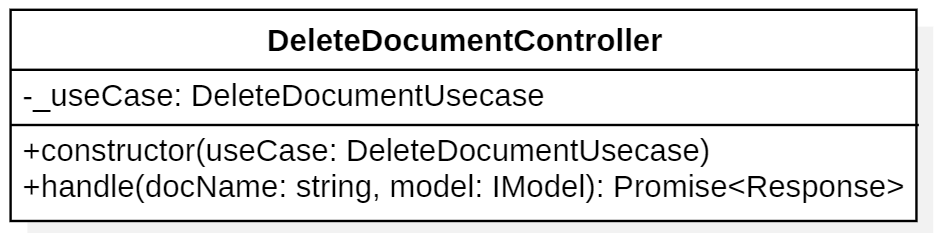
\includegraphics[width=0.6\textwidth]{DeleteDocumentController.png}
    \caption{UML della classe DeleteDocumentController}
\end{figure}

\subsubsection{UpdateDocumentController}
\textbf{Decoratori}
\begin{itemize}
    \item \textit{@injectable()}: decoratore per la Dependency Injection mediante Tsyringe.
\end{itemize}
\textbf{Attributi}
\begin{itemize}
    \item private readonly \textit{\_useCase: UpdateDocumentUsecase}.
\end{itemize}
\textbf{Metodi}
\begin{itemize}
    \item \textit{handle(docName: string, model: IModel, updatedMetadas: Metadatas): Promise<Response>}.
\end{itemize}
\textbf{Descrizione}\\
Questa classe controller, chiamata tramite la server action updateDocument, gestisce la chiamata al UpdateDocumentUsecase per aggiornare i tag e i metadati associati ad un documento, passando una \textit{string} docName, una \textit{string} model e dei metadati updatedMetadas, che rappresentano il nome del documento da aggiornare, il modello di appartenenza e il nuovo valore del tag di visibilità associato.\\ \\
\textbf{Dipendenze}
\begin{itemize}
    \item UpdateDocumentUsecase.
\end{itemize}

\begin{figure}[h!]
    \centering  
    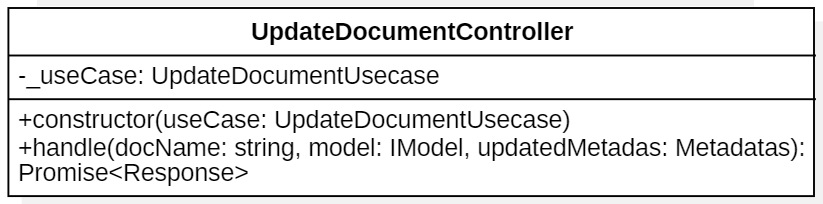
\includegraphics[width=0.7\textwidth]{UpdateDocumentController.png}
    \caption{UML della classe UpdateDocumentController}
\end{figure}

\subsubsection{GetDocumentContentController}
\textbf{Decoratori}
\begin{itemize}
    \item \textit{@injectable()}: decoratore per la Dependency Injection mediante Tsyringe.
\end{itemize}
\textbf{Attributi}
\begin{itemize}
    \item private readonly \textit{\_useCase: GetDocumentContentUsecase}.
\end{itemize}
\textbf{Metodi}
\begin{itemize}
    \item \textit{handle(docName: string, model: IModel): Promise<Response>}.
\end{itemize}
\textbf{Descrizione}\\
Questa classe controller, chiamata tramite la server action getDocumentContent, gestisce la chiamata al GetDocumentContentUsecase per recuperare dal sistema il link di visualizzazione di un documento, passando una \textit{string} docName e un \textit{IModel} (stringa con il nome di un modello) model, che rappresentano il nome del documento di interesse e il modello che presenta il documento.\\ \\
\textbf{Dipendenze}
\begin{itemize}
    \item GetDocumentContentUsecase.
\end{itemize}

\begin{figure}[h!]
    \centering  
    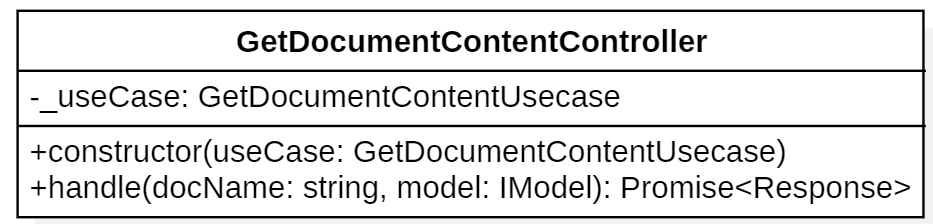
\includegraphics[width=0.6\textwidth]{GetDocumentContentController.png}
    \caption{UML della classe GetDocumentContentController}
\end{figure}

\subsubsection{GetDocumentsController}
\textbf{Decoratori}
\begin{itemize}
    \item \textit{@injectable()}: decoratore per la Dependency Injection mediante Tsyringe.
\end{itemize}
\textbf{Attributi}
\begin{itemize}
    \item private readonly \textit{\_useCase: GetDocumentsUsecase}.
\end{itemize}
\textbf{Metodi}
\begin{itemize}
    \item \textit{handle(model: IModel): Promise<Response>}.
\end{itemize}
\textbf{Descrizione}\\
Questa classe controller, chiamata tramite la server action getDocuments, gestisce la chiamata al GetDocumentsUsecase per recuperare le informazioni dei documenti quali nome, data di ultima modifica e dimensione, passando una \textit{string} model, che rappresenta il nome del modello da cui recuperare i documenti.\\ \\
\textbf{Dipendenze}
\begin{itemize}
    \item GetDocumentsUsecase.
\end{itemize}

\begin{figure}[h!]
    \centering  
    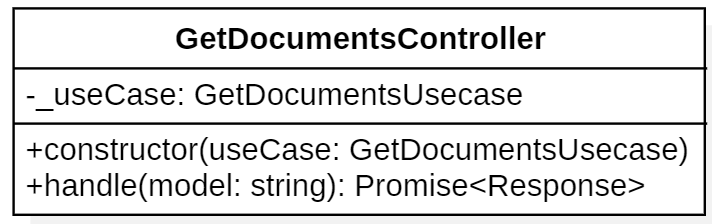
\includegraphics[width=0.6\textwidth]{GetDocumentsController.png}
    \caption{UML della classe GetDocumentsController}
\end{figure}

\subsubsection{AddChatController}
\textbf{Decoratori}
\begin{itemize}
    \item \textit{@injectable()}: decoratore per la Dependency Injection mediante Tsyringe.
\end{itemize}
\textbf{Attributi}
\begin{itemize}
    \item private readonly \textit{\_useCase: AddChatUsecase}.
\end{itemize}
\textbf{Metodi}
\begin{itemize}
    \item \textit{handle(title: string): Promise<Response>}.
\end{itemize}
\textbf{Descrizione}\\
Questa classe controller, chiamata tramite la server action addChat, gestisce la chiamata al AddChatUsecase per creare una nuova sessione di conversazione, passando una \textit{string} title che rappresenta il nome che prenderà quella sessione.\\ \\
\textbf{Dipendenze}
\begin{itemize}
    \item AddChatUsecase.
\end{itemize}

\begin{figure}[h!]
    \centering  
    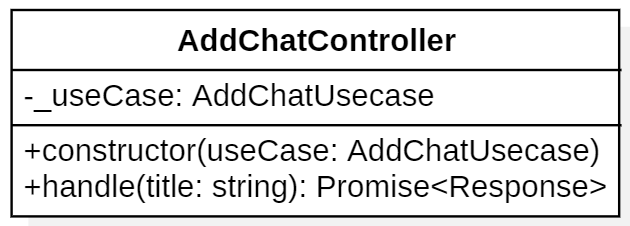
\includegraphics[width=0.6\textwidth]{AddChatController.png}
    \caption{UML della classe AddChatController}
\end{figure}

\subsubsection{AddChatMessagesController}
\textbf{Decoratori}
\begin{itemize}
    \item \textit{@injectable()}: decoratore per la Dependency Injection mediante Tsyringe.
\end{itemize}
\textbf{Attributi}
\begin{itemize}
    \item private readonly \textit{\_useCase: AddChatMessagesUsecase}.
\end{itemize}
\textbf{Metodi}
\begin{itemize}
    \item \textit{handle(messages: ICustomMessages): Promise<Response>}.
\end{itemize}
\textbf{Descrizione}\\
Questa classe controller, chiamata tramite la server action addChatMessages, gestisce la chiamata al AddChatMessagesUsecase dove viene passato un nuovo messaggio scambiato in una sessione (messages: \textit{ICustomMessages}) da aggiungere nel database.\\ \\
\textbf{Dipendenze}
\begin{itemize}
    \item AddChatMesagesUsecase.
\end{itemize}

\begin{figure}[h!]
    \centering  
    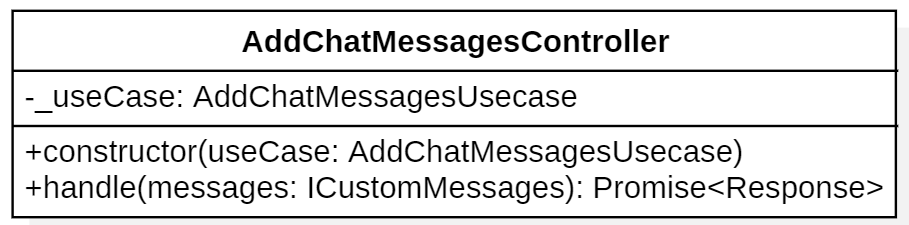
\includegraphics[width=0.6\textwidth]{AddChatMessagesController.png}
    \caption{UML della classe AddChatMessagesController}
\end{figure}

\subsubsection{DeleteAllChatController}
\textbf{Decoratori}
\begin{itemize}
    \item \textit{@injectable()}: decoratore per la Dependency Injection mediante Tsyringe.
\end{itemize}
\textbf{Attributi}
\begin{itemize}
    \item private readonly \textit{\_useCase: DeleteAllChatUsecase}.
\end{itemize}
\textbf{Metodi}
\begin{itemize}
    \item \textit{handle(): Promise<Response>}.
\end{itemize}
\textbf{Descrizione}\\
Questa classe controller, chiamata tramite la server action deleteAllChat, gestisce la chiamata al DeleteAllChatUsecase per rimuovere nel database tutte le sessioni e le chat history relative.\\ \\
\textbf{Dipendenze}
\begin{itemize}
    \item DeleteAllChatUsecase.
\end{itemize}

\begin{figure}[h!]
    \centering  
    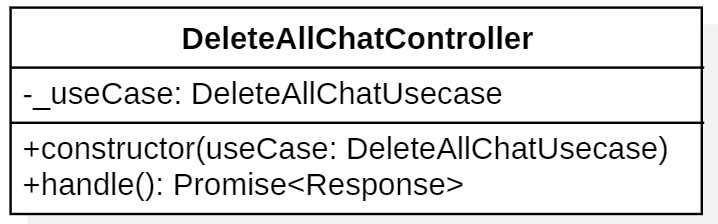
\includegraphics[width=0.6\textwidth]{DeleteAllChatController.png}
    \caption{UML della classe DeleteAllChatController}
\end{figure}

\subsubsection{DeleteChatController}
\textbf{Decoratori}
\begin{itemize}
    \item \textit{@injectable()}: decoratore per la Dependency Injection mediante Tsyringe.
\end{itemize}
\textbf{Attributi}
\begin{itemize}
    \item private readonly \textit{\_useCase: DeleteChatUsecase}.
\end{itemize}
\textbf{Metodi}
\begin{itemize}
    \item \textit{handle(id: number): Promise<Response>}.
\end{itemize}
\textbf{Descrizione}\\
Questa classe controller, chiamata tramite la server action deleteChat, gestisce la chiamata al DeleteChatUsecase per rimuovere dal database una particolare sessione, identificata dal \textit{number} id, e la chat history relativa.\\ \\
\textbf{Dipendenze}
\begin{itemize}
    \item DeleteChatUsecase.
\end{itemize}

\begin{figure}[h!]
    \centering  
    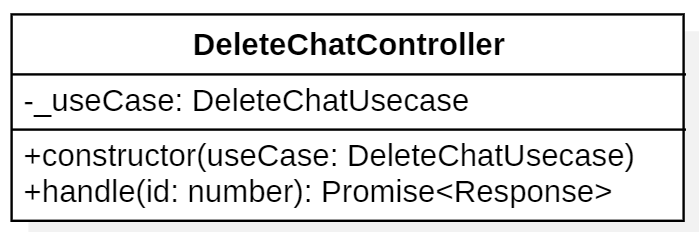
\includegraphics[width=0.6\textwidth]{DeleteChatController.png}
    \caption{UML della classe DeleteChatController}
\end{figure}

\subsubsection{GetChatMessagesController}
\textbf{Decoratori}
\begin{itemize}
    \item \textit{@injectable()}: decoratore per la Dependency Injection mediante Tsyringe.
\end{itemize}
\textbf{Attributi}
\begin{itemize}
    \item private readonly \textit{\_useCase: GetChatMessagesUsecase}.
\end{itemize}
\textbf{Metodi}
\begin{itemize}
    \item \textit{handle(id: number): Promise<Response>}.
\end{itemize}
\textbf{Descrizione}\\
Questa classe controller, chiamata tramite la server action getChatMessages, gestisce la chiamata al GetChatMessagesUsecase per recuperare dal database la chat history di una particolare sessione, identificata dal \textit{number} id.\\ \\
\textbf{Dipendenze}
\begin{itemize}
    \item GetChatMessagesUsecase.
\end{itemize}

\begin{figure}[h!]
    \centering  
    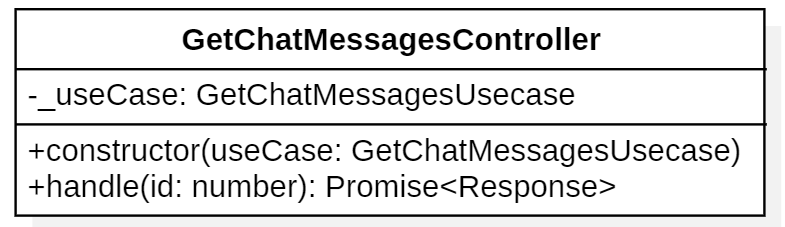
\includegraphics[width=0.6\textwidth]{GetChatMessagesController.png}
    \caption{UML della classe GetChatMessagesController}
\end{figure}

\subsubsection{GetChatsController}
\textbf{Decoratori}
\begin{itemize}
    \item \textit{@injectable()}: decoratore per la Dependency Injection mediante Tsyringe.
\end{itemize}
\textbf{Attributi}
\begin{itemize}
    \item private readonly \textit{\_useCase: GetChatsUsecase}.
\end{itemize}
\textbf{Metodi}
\begin{itemize}
    \item \textit{handle(): Promise<Response}>.
\end{itemize}
\textbf{Descrizione}\\
Questa classe controller, chiamata tramite la server action getChats, gestisce la chiamata al GetChatsUsecase per recuperare dal database le sessioni di conversazione attive nel sistema.\\ \\
\textbf{Dipendenze}
\begin{itemize}
    \item GetChatsUsecase.
\end{itemize}

\begin{figure}[h!]
    \centering  
    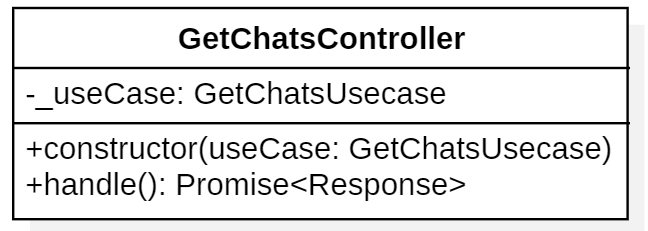
\includegraphics[width=0.6\textwidth]{GetChatsController.png}
    \caption{UML della classe GetChatsController}
\end{figure}

\newpage

\subsection{Use Cases} \label{subsec:usecases}
\subsubsection{AddDocumentUsecase}
\textbf{Decoratori}
\begin{itemize}
    \item \textit{@injectable()}: decoratore per la Dependency Injection mediante Tsyringe.
\end{itemize}
\textbf{Attributi}
\begin{itemize}[itemsep=-4pt]
    \item private readonly \textit{\_documentRepository: IDocumentRepository};
    \item private readonly \textit{\_embeddingRepository: IEmbeddingRepository};
    \item private readonly \textit{\_embeddingsFunction}.
\end{itemize}
\textbf{Metodi}
\begin{itemize}
    \item \textit{execute(file: File, model: IModel)}.
\end{itemize}
\textbf{Descrizione}\\
Questo use case, chiamato dal AddDocumentController, contiene la business logic relativa alle operazioni per aggiungere un nuovo documento nel sistema. Ricevuto il file e la \textit{string} model, gestisce la chiamata al DocumentRepository per aggiungere il nuovo documento. Dopo aver effettuato il parsing del contenuto del documento e averlo diviso per pagine, viene effettuato l'embedding del testo utilizzando l'embedding function determinata dal modello desiderato. Una volta completato questo processo, mapando gli embedding con il nome del documento, i metadati associati e il suo file, viene chiamato anche l'EmbeddingRepository per lo storage dei vettori sul database vettoriale.\\
Presenta un riferimento a delle interfacce IDocumentRepository e IEmbeddingRepository, le cui implementazioni concrete sono DocumentRepository e EmbeddingRepository, che espongono i metodi per lavorare sulle fonti dei dati presenti nel database.\\ \\
\textbf{Dipendenze}
\begin{itemize}[itemsep=-4pt]
    \item IDocumentRepository;
    \item IEmbeddingRepository.
\end{itemize}
\textbf{Requisiti associati}
\begin{itemize}[itemsep=-4pt]
    \item RFO-29;
    \item RIO-1;
    \item RIO-2;
    \item RIO-3;
    \item RIO-4.
\end{itemize}

\begin{figure}[h!]
    \centering  
    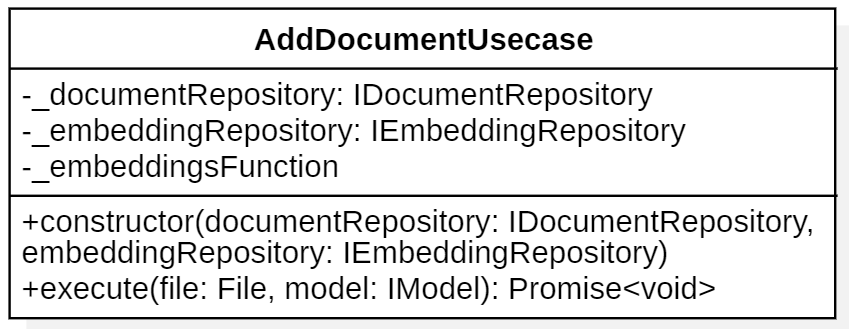
\includegraphics[width=0.5\textwidth]{AddDocumentUsecase.png}
    \caption{UML della classe AddDocumentUsecase}
\end{figure}

\subsubsection{DeleteDocumentUsecase}
\textbf{Decoratori}
\begin{itemize}
    \item \textit{@injectable()}: decoratore per la Dependency Injection mediante Tsyringe.
\end{itemize}
\textbf{Attributi}
\begin{itemize}[itemsep=-4pt]
    \item private readonly \textit{\_documentRepository: IDocumentRepository};
    \item private readonly \textit{\_embeddingRepository: IEmbeddingRepository}.
\end{itemize}
\textbf{Metodi}
\begin{itemize}
    \item \textit{execute(docName: string, model: IModel)}.
\end{itemize}
\textbf{Descrizione}\\
Questo use case, chiamato dal DeleteDocumentController, contiene la business logic relativa alle operazioni per eliminare uno specifico documento dal sistema. Ricevute le \textit{string} docName e model, gestisce la chiamata al DocumentRepository e all'EmbeddingRepository per rimuovere nuovo documento.\\
Dopo aver effettuato la chiamata al DocumentRepository per richiedere l'eliminazione del documento dal database MinIO, richiede l'id degli embedding da rimuovere all'EmbeddingRepository, per poi richiedere l'eliminazione dei vettori identificati da essi alla medesima classe repository.\\
Presenta un riferimento a delle interfacce IDocumentRepository e IEmbeddingRepository, le cui implementazioni concrete sono DocumentRepository e EmbeddingRepository, che espongono i metodi per lavorare sulle fonti dei dati presenti nel database. \\ \\
\textbf{Dipendenze}
\begin{itemize}[itemsep=-4pt]
    \item IDocumentRepository;
    \item IEmbeddingRepository.
\end{itemize}
\textbf{Requisiti associati}
\begin{itemize}
    \item RFO-27.
\end{itemize}

\begin{figure}[h!]
    \centering  
    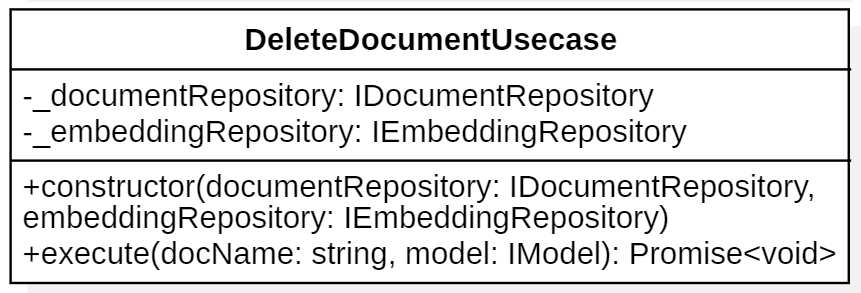
\includegraphics[width=0.5\textwidth]{DeleteDocumentUsecase.png}
    \caption{UML della classe DeleteDocumentUsecase}
\end{figure}

\subsubsection{UpdateDocumentUsecase}
\textbf{Decoratori}
\begin{itemize}
    \item \textit{@injectable()}: decoratore per la Dependency Injection mediante Tsyringe.
\end{itemize}
\textbf{Attributi}
\begin{itemize}[itemsep=-4pt]
    \item private readonly \textit{\_documentRepository: IDocumentRepository};
    \item private readonly \textit{\_embeddingRepository: IEmbeddingRepository}.
\end{itemize}
\textbf{Metodi}
\begin{itemize}
    \item \textit{execute(docName: string, model: IModel, updatedMetadas: Metadatas)}.
\end{itemize}
\textbf{Descrizione}\\
Questo use case, chiamato dal UpdateDocumentController, contiene la business logic relativa alle operazioni per aggiornare i tag e i metadati, relativi alla visibilità, di uno specifico documento. Ricevute le \textit{string} docName e model e i nuovi metadati updatedMetadas, gestisce la chiamata al DocumentRepository e all'EmbeddingRepository per aggiornare i valori.\\
Dopo aver effettuato la chiamata al DocumentRepository per richiedere l'aggiornamento del tag di visibilità del documento nel database MinIO, richiede l'id degli embedding da modificare all'EmbeddingRepository, per poi richiedere la modifica del metadato visibility dei vettori identificati da essi alla medesima classe repository.\\
Presenta un riferimento a delle interfacce IDocumentRepository e IEmbeddingRepository, le cui implementazioni concrete sono DocumentRepository e EmbeddingRepository, che espongono i metodi per lavorare sulle fonti dei dati presenti nel database.\\ \\
\textbf{Dipendenze}
\begin{itemize}[itemsep=-4pt]
    \item IDocumentRepository;
    \item IEmbeddingRepository.
\end{itemize}
\textbf{Requisiti associati}
\begin{itemize}[itemsep=-4pt]
    \item RFZ-15;
    \item RFZ-16;
    \item RFD-36;
    \item RFD-37.
\end{itemize}

\begin{figure}[h!]
    \centering  
    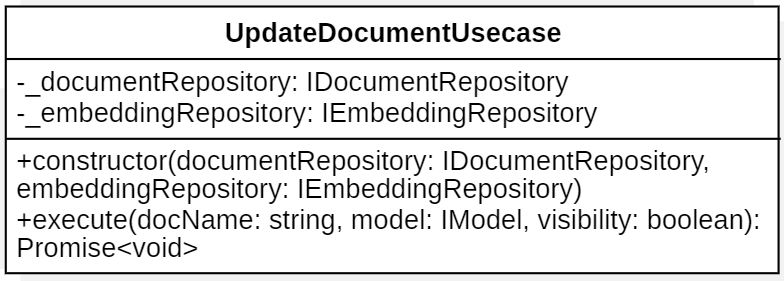
\includegraphics[width=0.5\textwidth]{UpdateDocumentUsecase.png}
    \caption{UML della classe UpdateDocumentUsecase}
\end{figure}

\subsubsection{GetDocumentContentUsecase}
\textbf{Decoratori}
\begin{itemize}
    \item \textit{@injectable()}: decoratore per la Dependency Injection mediante Tsyringe.
\end{itemize}
\textbf{Attributi}
\begin{itemize}
    \item private readonly \textit{\_documentRepository : IDocumentRepository}.
\end{itemize}
\textbf{Metodi}
\begin{itemize}
    \item \textit{execute(docName: string, model: IModel)}.
\end{itemize}
\textbf{Descrizione}\\
Questo use case, chiamato dal GetDocumentContentController, contiene la business logic relativa alle operazioni per ottenere il link di visualizzazione di uno specifico documento dal sistema. Ricevute le \textit{string} docName e model, gestisce la chiamata al DocumentRepository per recuperare tale informazione.\\
Presenta un riferimento ad un'interfaccia IDocumentRepository , la cui implementazione concreta è DocumentRepository, che espone i metodi per lavorare sulle fonti dei dati presenti nel database.\\ \\
\textbf{Dipendenze}
\begin{itemize}
    \item IDocumentRepository.
\end{itemize}
\textbf{Requisiti associati}
\begin{itemize}[itemsep=-4pt]
    \item RFO-8;
    \item RFO-55.
\end{itemize}

\begin{figure}[h!]
    \centering  
    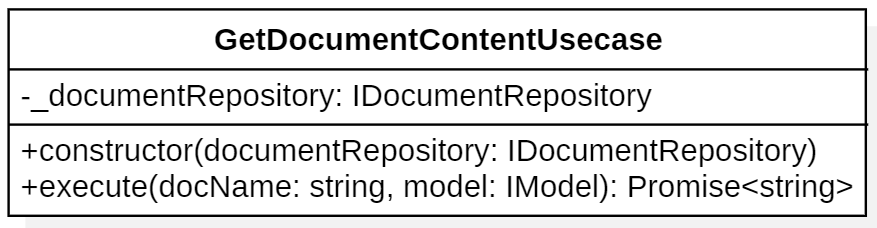
\includegraphics[width=0.48\textwidth]{GetDocumentContentUsecase.png} %non toccare questo valore, lo so che non si vede molto, ma se viene modificato crolla tutta la renderizzazione della pagina
    \caption{UML della classe GetDocumentContentUsecase}
\end{figure}

\subsubsection{GetDocumentsUsecase}
\textbf{Decoratori}
\begin{itemize}
    \item \textit{@injectable()}: decoratore per la Dependency Injection mediante Tsyringe.
\end{itemize}
\textbf{Attributi}
\begin{itemize}[itemsep=-4pt]
    \item private readonly \textit{\_documentRepository : IDocumentRepository}.
\end{itemize}
\textbf{Metodi}
\begin{itemize}
    \item \textit{execute(model: IModel) : Promise<Document[]>}.
\end{itemize}
\textbf{Descrizione}\\
Questo use case, chiamato dal GetDocumentsController, contiene la business logic relativa alle operazioni per ottenere le informazioni dei documenti presenti nel sistema. Ricevuto il model, gestisce la chiamata al DocumentRepository per recuperare le informazioni dei documenti presenti in quello specifico modello.\\
Presenta un riferimento ad un'interfaccia IDocumentRepository , la cui implementazione concreta è DocumentRepository, che espone i metodi per lavorare sulle fonti dei dati presenti nel database.\\ \\
\textbf{Dipendenze}
\begin{itemize}
    \item IDocumentRepository.
\end{itemize}
\textbf{Requisiti associati}
\begin{itemize}[itemsep=-4pt]
    \item RFO-4;
    \item RFO-5;
    \item RFO-6;
    \item RFZ-7;
    \item RFD-9;
    \item RFO-10.
\end{itemize}

\begin{figure}[h!]
    \centering  
    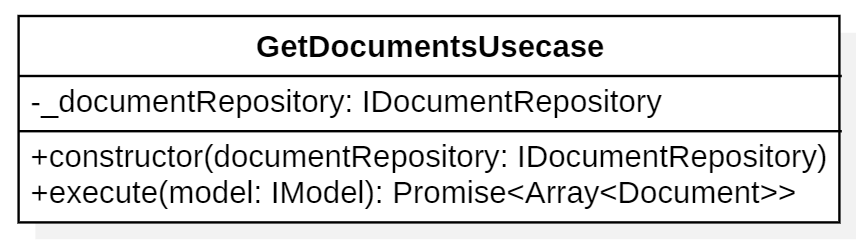
\includegraphics[width=0.5\textwidth]{GetDocumentsUsecase.png}
    \caption{UML della classe GetDocumentsUsecase}
\end{figure}

\subsubsection{AddChatMessagesUsecase}
\textbf{Decoratori}
\begin{itemize}
    \item \textit{@injectable()}: decoratore per la Dependency Injection mediante Tsyringe.
\end{itemize}
\textbf{Attributi}
\begin{itemize}
    \item private readonly \textit{\_chatRepository: IChatRepository}.
\end{itemize}
\textbf{Metodi}
\begin{itemize}
    \item \textit{execute(messages: ICustomMessages): Promise<void>}.
\end{itemize}
\textbf{Descrizione}\\
Questo use case, chiamato dal AddChatMessagesController, contiene la business logic relativa alle operazioni per aggiungere le informazioni dei messaggi scritti, definiti dall'\textit{ICustomMessages}. Ricevuto il messages, gestisce la chiamata al ChatRepository per richiedere il salvataggio del dato.\\
Presenta un riferimento ad un'interfaccia IChatRepository , la cui implementazione concreta è ChatRepository, che espone i metodi per lavorare sulle fonti dei dati presenti nel database.\\ \\
\textbf{Dipendenze}
\begin{itemize}
    \item IChatRepository.
\end{itemize}
\textbf{Requisiti associati}
\begin{itemize}[itemsep=-4pt]
    \item RFO-52.
\end{itemize}

\begin{figure}[h!]
    \centering  
    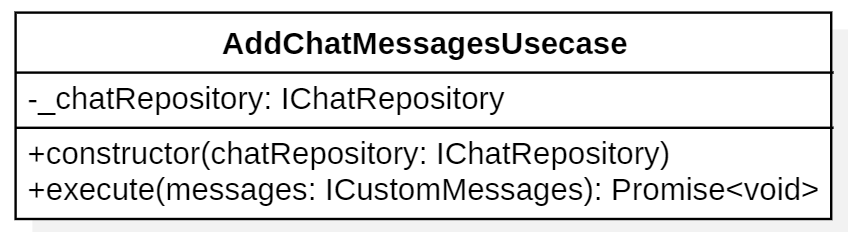
\includegraphics[width=0.5\textwidth]{AddChatMessagesUsecase.png}
    \caption{UML della classe AddChatMessagesUsecase}
\end{figure}

\subsubsection{AddChatUsecase}
\textbf{Decoratori}
\begin{itemize}
    \item \textit{@injectable()}: decoratore per la Dependency Injection mediante Tsyringe.
\end{itemize}
\textbf{Attributi}
\begin{itemize}
    \item private readonly \textit{\_chatRepository: IChatRepository}.
\end{itemize}
\textbf{Metodi}
\begin{itemize}
    \item \textit{execute(title: string): Promise<void>}.
\end{itemize}
\textbf{Descrizione}\\
Questo use case, chiamato dal AddChatController, contiene la business logic relativa alle operazioni per aggiungere una nuova sessione di conversazione nel sistema, che avrà un nome definito dalla \textit{string} title. Ricevuto questo title, gestisce la chiamata al ChatRepository per richiedere la creazione della nuova sessione.\\
Presenta un riferimento ad un'interfaccia IChatRepository , la cui implementazione concreta è ChatRepository, che espone i metodi per lavorare sulle fonti dei dati presenti nel database.\\ \\
\textbf{Dipendenze}
\begin{itemize}
    \item IChatRepository.
\end{itemize}
\textbf{Requisiti associati}
\begin{itemize}
    \item RFD-48.
\end{itemize}

\begin{figure}[h!]
    \centering  
    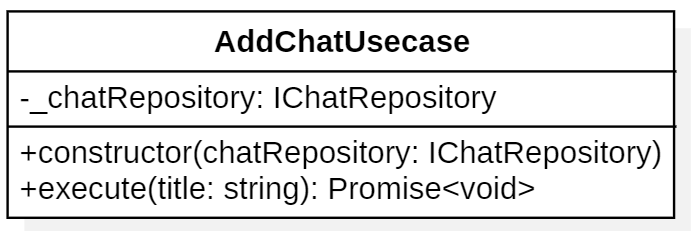
\includegraphics[width=0.5\textwidth]{AddChatUsecase.png}
    \caption{UML della classe AddChatUsecase}
\end{figure}

\subsubsection{DeleteAllChatUsecase}
\textbf{Decoratori}
\begin{itemize}
    \item \textit{@injectable()}: decoratore per la Dependency Injection mediante Tsyringe.
\end{itemize}
\textbf{Attributi}
\begin{itemize}
    \item private readonly \textit{\_chatRepository: IChatRepository}.
\end{itemize}
\textbf{Metodi}
\begin{itemize}
    \item \textit{execute(): Promise<number>.}
\end{itemize}
\textbf{Descrizione}\\
Questo use case, chiamato dal DeleteAllChatController, contiene la business logic relativa alle operazioni per eliminare dal database tutte le informazioni relative alle sessioni di conversazione attive, incluse le chat history ad esse associate.\\
Presenta un riferimento ad un'interfaccia IChatRepository , la cui implementazione concreta è ChatRepository, che espone i metodi per lavorare sulle fonti dei dati presenti nel database.\\ \\
\textbf{Dipendenze}
\begin{itemize}
    \item IChatRepository.
\end{itemize}
\textbf{Requisiti associati}
\begin{itemize}[itemsep=-4pt]
    \item RFD-50;
    \item RFD-51.
\end{itemize}

\begin{figure}[h!]
    \centering  
    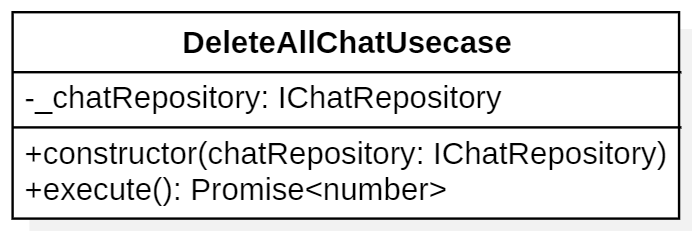
\includegraphics[width=0.5\textwidth]{DeleteAllChatUsecase.png}
    \caption{UML della classe DeleteAllChatUsecase}
\end{figure}

\subsubsection{DeleteChatUsecase}
\textbf{Decoratori}
\begin{itemize}
    \item \textit{@injectable()}: decoratore per la Dependency Injection mediante Tsyringe.
\end{itemize}
\textbf{Attributi}
\begin{itemize}
    \item private readonly \textit{\_chatRepository: IChatRepository}.
\end{itemize}
\textbf{Metodi}
\begin{itemize}
    \item \textit{execute(id: number): Promise<void>}.
\end{itemize}
\textbf{Descrizione}\\
Questo use case, chiamato dal DeleteChatController, contiene la business logic relativa alle operazioni per eliminare dal database tutte le informazioni relative ad una particolare sessione di conversazione, definita dal \textit{number} id, e alla sua chat history. Ricevuto l'id, gestisce la chiamata al ChatRepository per richiedere l'eliminazione della sessione.\\
Presenta un riferimento ad un'interfaccia IChatRepository , la cui implementazione concreta è ChatRepository, che espone i metodi per lavorare sulle fonti dei dati presenti nel database.\\ \\
\textbf{Dipendenze}
\begin{itemize}
    \item IChatRepository.
\end{itemize}
\textbf{Requisiti associati}
\begin{itemize}[itemsep=-4pt]
    \item RFD-53;
    \item RFD-54.
\end{itemize}

\begin{figure}[h!]
    \centering  
    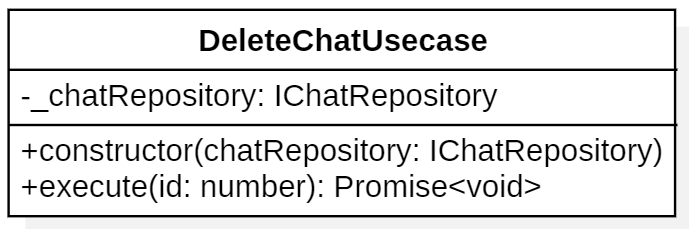
\includegraphics[width=0.5\textwidth]{DeleteChatUsecase.png}
    \caption{UML della classe DeleteChatUsecase}
\end{figure}

\subsubsection{GetChatMessagesUsecase}
\textbf{Decoratori}
\begin{itemize}
    \item \textit{@injectable()}: decoratore per la Dependency Injection mediante Tsyringe.
\end{itemize}
\textbf{Attributi}
\begin{itemize}
    \item private readonly \textit{\_chatRepository: IChatRepository}.
\end{itemize}
\textbf{Metodi}
\begin{itemize}
    \item \textit{execute(id: number): Promise<allMessages: Message[], source: MessageSource>}.
\end{itemize}
\textbf{Descrizione}\\
Questo use case, chiamato dal GetChatMessagesController, contiene la business logic relativa alle operazioni per ottenere dal database la chat history relativa ad una particolare sessione di conversazione, definita dal \textit{number} id. Ricevuto l'id, gestisce la chiamata al ChatRepository per il recupero dei messaggi.\\
Presenta un riferimento ad un'interfaccia IChatRepository , la cui implementazione concreta è ChatRepository, che espone i metodi per lavorare sulle fonti dei dati presenti nel database.\\ \\
\textbf{Dipendenze}
\begin{itemize}
    \item IChatRepository.
\end{itemize}
\textbf{Requisiti associati}
\begin{itemize}
    \item RFO-52.
\end{itemize}

\begin{figure}[h!]
    \centering  
    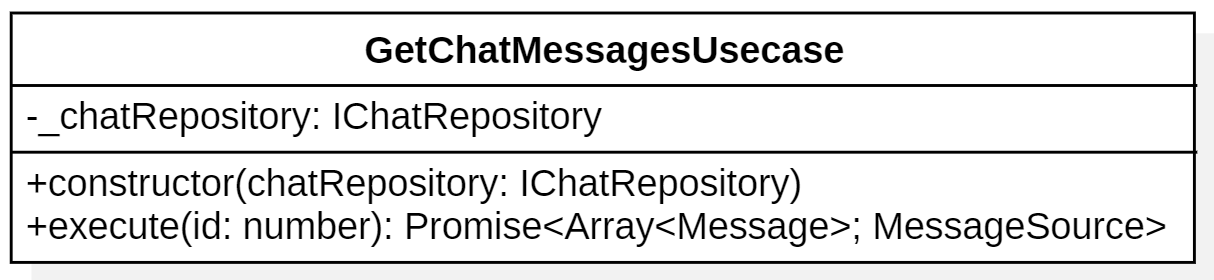
\includegraphics[width=0.5\textwidth]{GetChatMessagesUsecase.png}
    \caption{UML della classe GetChatMessagesUsecase}
\end{figure}

\subsubsection{GetChatsUsecase}
\textbf{Decoratori}
\begin{itemize}
    \item \textit{@injectable()}: decoratore per la Dependency Injection mediante Tsyringe.
\end{itemize}
\textbf{Attributi}
\begin{itemize}
    \item private readonly \textit{\_chatRepository: IChatRepository}.
\end{itemize}
\textbf{Metodi}
\begin{itemize}
    \item \textit{execute(): Promise<Chat[]>}.
\end{itemize}
\textbf{Descrizione}\\
Questo use case, chiamato dal GetChatsController, contiene la business logic relativa alle operazioni per ottenere dal database le informazioni relative alle sessioni di conversazione salvate e attive nel sistema.\\
Presenta un riferimento ad un'interfaccia IChatRepository , la cui implementazione concreta è ChatRepository, che espone i metodi per lavorare sulle fonti dei dati presenti nel database.\\ \\
\textbf{Dipendenze}
\begin{itemize}
    \item IChatRepository.
\end{itemize}
\textbf{Requisiti associati}
\begin{itemize}
    \item RFD-49.
\end{itemize}

\begin{figure}[h!]
    \centering  
    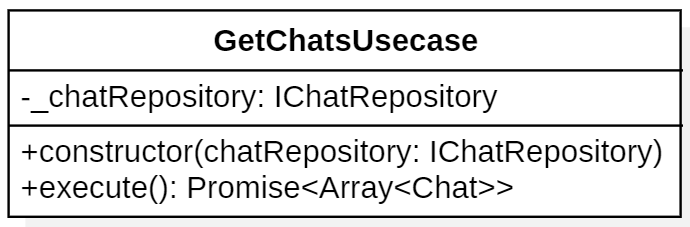
\includegraphics[width=0.5\textwidth]{GetChatsUsecase.png}
    \caption{UML della classe GetChatsUsecase}
\end{figure}

\subsection{Repositories} \label{subsec:repositories}
\subsubsection{DocumentRepository}
\textbf{Decoratori}
\begin{itemize}
    \item \textit{@injectable()}: decoratore per la Dependency Injection mediante Tsyringe.
\end{itemize}
\textbf{Attributi}
\begin{itemize}
    \item private \textit{\_documentDataSource: IDocumentDataSource}.
\end{itemize}
\textbf{Metodi}
\begin{itemize}[itemsep=-4pt]
    \item \textit{addDocument(doc: Document, model: IModel): Promise<void>};
    \item \textit{deleteDocument(docName: string, model: IModel): Promise<void>};
    \item \textit{updateDocument(docName: string, model: IModel, tag: Metadatas): Promise<void>};
    \item \textit{getDocuments(model: IModel): Promise<Document[]>};
    \item \textit{getDocumentContent(docName: string, model: IModel): Promise<string>}. 
\end{itemize}
\textbf{Descrizione}\\
La classe DocumentRepository, utilizzata dagli use cases AddDocument, DeleteDocument, UpdateDocument, GetDocumentContent e GetDocuments, espone i metodi con cui interfacciarsi alle fonti dei dati per il recupero dei dati necessari alla logica di business per aggiunta, rimozione, modifica e lettura dei documenti.\\
Presenta un riferimento ad un'interfaccia IDocumentDataSource, la cui implementazione concreta è MinioDataSource che espone i metodi per lavorare sui dati presenti nel database.\\ \\
\textbf{Dipendenze}
\begin{itemize}
    \item IDocumentDataSource.
\end{itemize}

\begin{figure}[h!]
    \centering  
    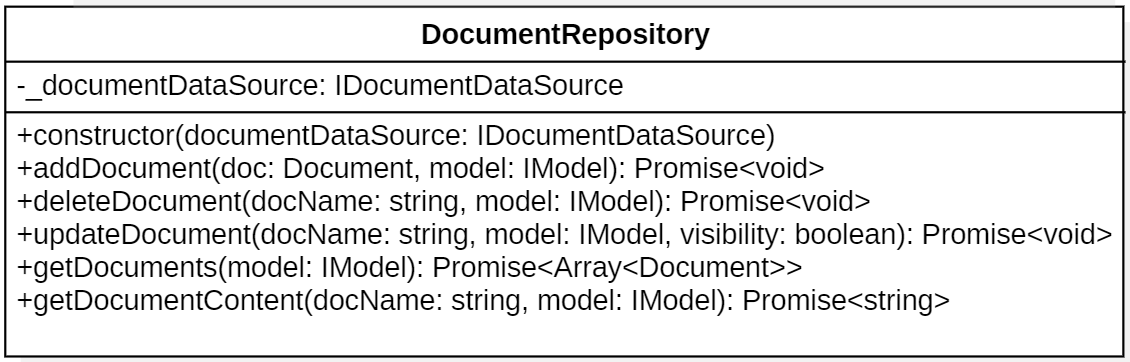
\includegraphics[width=0.7\textwidth]{DocumentRepository.png}
    \caption{UML della classe DocumentRepository}
\end{figure}

\subsubsection{EmbeddingRepository}
\textbf{Decoratori}
\begin{itemize}
    \item \textit{@injectable()}: decoratore per la Dependency Injection mediante Tsyringe.
\end{itemize}
\textbf{Attributi}
\begin{itemize}
    \item private \textit{\_embeddingsDataSource: IEmbeddingDataSource}.
\end{itemize}
\textbf{Metodi}
\begin{itemize}[itemsep=-4pt]
    \item \textit{addEmbedding(embeddings: Embeddings, model: IModel): Promise<void>};
    \item \textit{deleteEmbedding(ids: string[], model: IModel): Promise<void>};
    \item \textit{updateMetadatas(metadatas: Metadatas, model: IModel, ids: string[]): Promise<void>};
    \item \textit{getIdsEmbedding(docName: string, model: IModel): Promise<any>}.
\end{itemize}
\textbf{Descrizione}\\
La classe EmbeddingRepository, utilizzata dagli use cases AddDocument e DeleteDocument, espone i metodi con cui interfacciarsi alle fonti dei dati per il recupero dei dati necessari all'aggiunta ed eliminazione degli embedding di documenti.\\
Presenta un riferimento ad un'interfaccia IEmbeddingDataSource, la cui implementazione concreta è ChromaDataSource che espone i metodi per lavorare sui dati presenti nel vector database.\\ \\
\textbf{Dipendenze}
\begin{itemize}
    \item IEmbeddingDataSource.
\end{itemize}

\begin{figure}[h!]
    \centering  
    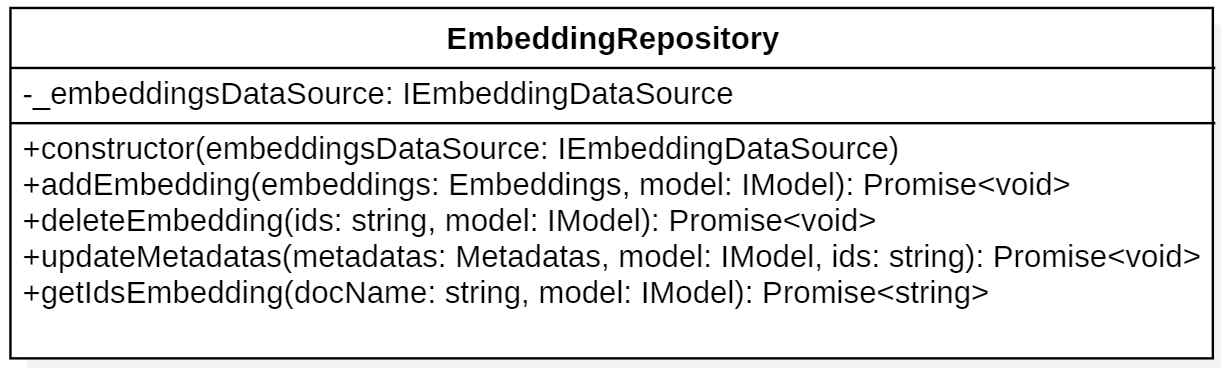
\includegraphics[width=0.7\textwidth]{EmbeddingRepository.png}
    \caption{UML della classe EmbeddingRepository}
\end{figure}

\newpage

\subsubsection{ChatRepository}
\textbf{Decoratori}
\begin{itemize}
    \item \textit{@injectable()}: decoratore per la Dependency Injection mediante Tsyringe.
\end{itemize}
\textbf{Attributi}
\begin{itemize}
    \item private \textit{\_chatDataSource: IChatDataSource}.
\end{itemize}
\textbf{Metodi}
\begin{itemize}[itemsep=-4pt]
    \item \textit{addChat(title: string): Promise<number>};
    \item \textit{addChatMessages(messages: ICustomMessages): Promise<void>};
    \item \textit{deleteAllChat(): Promise<void>};
    \item \textit{deleteChat(id: number): Promise<void>};
    \item \textit{getChatMessages(id: number): Promise<allMessages: Message[], source: MessageSource>};
    \item \textit{getChats(): Promise<Chat[]>}.
\end{itemize}
\textbf{Descrizione}\\
La classe ChatRepository, utilizzata dagli use cases AddChatMessages, AddChat, DeleteAllChat, DeleteChat, GetChatMessages e GetChats, espone i metodi con cui interfacciarsi alla fonte dei dati per il recupero delle informazioni necessarie alla logica di business per aggiunta, rimozione e recupero delle sessioni di conversazione e dei messaggi delle chat history ad esse associate.\\
Presenta un riferimento ad un'interfaccia IChatDataSource, la cui implementazione concreta è PostgresDataSource che espone i metodi per lavorare sui dati presenti nel database.\\ \\
\textbf{Dipendenze}
\begin{itemize}
    \item IChatDataSource.
\end{itemize}

\begin{figure}[h!]
    \centering  
    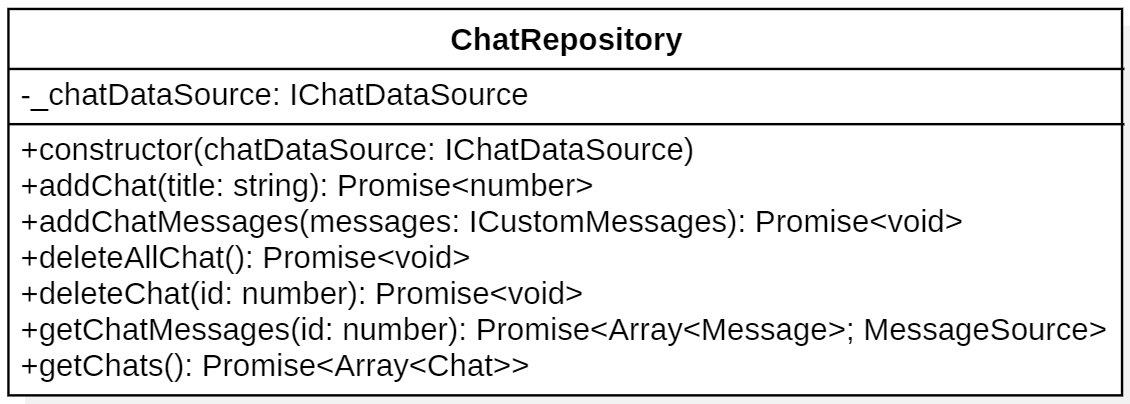
\includegraphics[width=0.6\textwidth]{ChatRepository.png}
    \caption{UML della classe ChatRepository}
\end{figure}
\subsection{Data Sources} \label{subsec:datasources}
\subsubsection{MinioDataSource}
\textbf{Decoratori}
\begin{itemize}
    \item \textit{@injectable()}: decoratore per la Dependency Injection mediante Tsyringe.
\end{itemize}
\textbf{Attributi}
\begin{itemize}
    \item private readonly \textit{\_db: S3}.
\end{itemize}
\textbf{Metodi}
\begin{itemize}[itemsep=-4pt]
    \item \textit{addOne(doc: Document, model: IModel): Promise<void>}\\
    Metodo per l'aggiunta di un nuovo documento nella collezione di un modello;
    \item \textit{deleteOne(docName: string, model: IModel): Promise<void>}\\
    Metodo per l'eliminazione di un documento dalla collezione di un modello;
    \item \textit{updateOne(docName:string, model:IModel, tag:Metadatas): Promise<void>}\\
    Metodo per l'aggiornamento del tag di visibilità di un documento di una particolare collezione;
    \item \textit{getAll(model: IModel): Promise<Document[]>}\\
    Metodo per recuperare i dati dei documenti contenuti in una collezione;
    \item \textit{getContent(docName: string, model: IModel): Promise<string>}\\
    Metodo per recuperare il link di visualizzazione di un documento.
\end{itemize}
\textbf{Descrizione}\\
La classe MinioDataSource implementa concretamente i metodi esposti all'interno di DocumentRepository. È lei ad operare sul database, tramite un attributo di tipo \textit{S3}.

\begin{figure}[h!]
    \centering  
    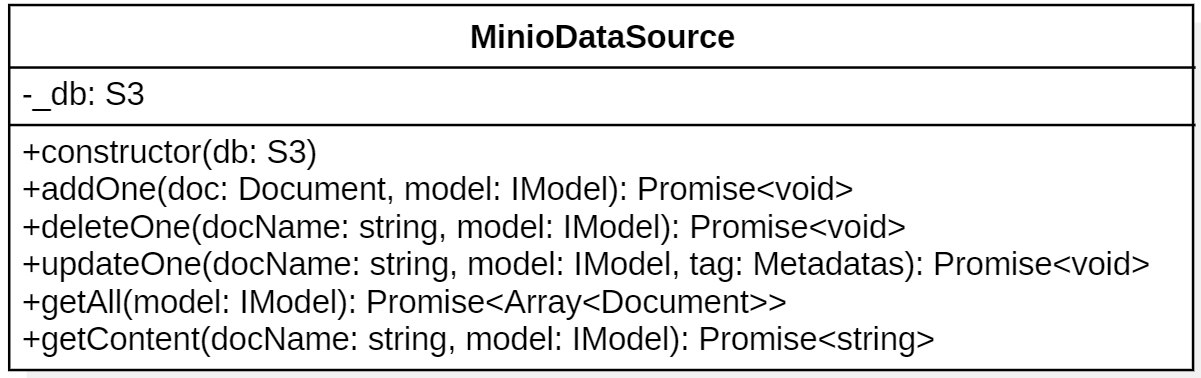
\includegraphics[width=0.6\textwidth]{MinioDataSource.png}
    \caption{UML della classe MinioDataSource}
\end{figure}

\newpage

\subsubsection{ChromaDataSource}
\textbf{Decoratori}
\begin{itemize}
    \item \textit{@injectable()}: decoratore per la Dependency Injection mediante Tsyringe.
\end{itemize}
\textbf{Attributi}
\begin{itemize}
    \item private readonly \textit{\_vDb: ChromaClient}.
\end{itemize}
\textbf{Metodi}
\begin{itemize}[itemsep=-4pt]
    \item \textit{addOne(embeddings: Embeddings, model: IModel): Promise<void>}\\
    Metodo per aggiungere gli embedding di un nuovo documento alla collezione di vettori di un modello;
    \item \textit{deleteOne(ids: string[], model: IModel): Promise<void>}\\
    Metodo per eliminare gli embedding di un preciso documento dalla collezione di vettori di un modello;
    \item \textit{updateOne(metadatas: Metadatas, model: IModel, ids: string[]): Promise<void>}\\
    Metodo per modificare i metadati degli embedding di un preciso documento in una collezione di vettori di un modello;
    \item\textit{getIds(docName: string, model: IModel): Promise<string>}\\
    Metodo per recuperare gli id di tutti i vettori che si riferiscono ad un preciso documento in una collezione di vettori di un modello.
\end{itemize}
\textbf{Descrizione}\\
La classe ChromaDataSource implementa concretamente i metodi esposti all'interno di EmbeddingRepository. È lei a svolgere le operazioni sul database vettoriale, tramite un attributo di tipo \textit{ChromaClient}.

\begin{figure}[h!]
    \centering  
    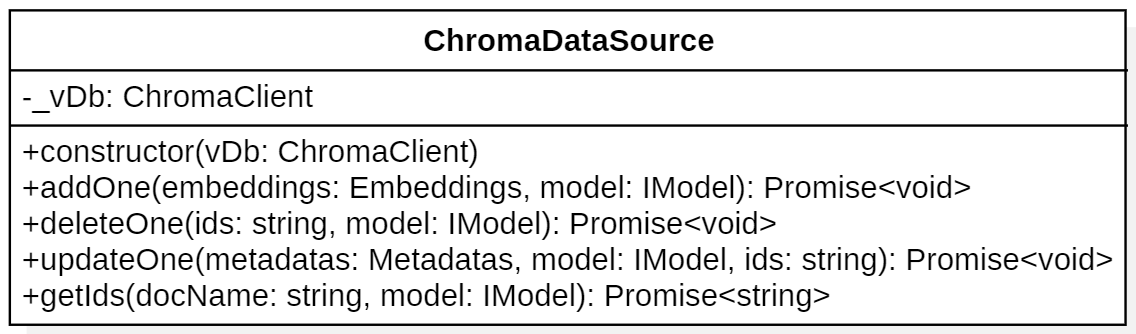
\includegraphics[width=0.6\textwidth]{ChromaDataSource.png}
    \caption{UML della classe ChromaDataSource}
\end{figure}

\newpage

\subsubsection{PostgresDataSource}
\textbf{Decoratori}
\begin{itemize}
    \item \textit{@injectable()}: decoratore per la Dependency Injection mediante Tsyringe.
\end{itemize}
\textbf{Attributi}
\begin{itemize}
    \item private readonly \textit{\_dB: Pool}.
\end{itemize}
\textbf{Metodi}
\begin{itemize}[itemsep=-4pt]
    \item \textit{addMessages(messages: ICustomMessages): Promise<void>}\\
    Metodo per salvare un messaggio nella relativa chat history di una conversazione;
    \item \textit{addOne(title: string): Promise<number>}\\
    Metodo per creare una nuova sessione di conversazione;
    \item \textit{deleteAll(): Promise<void>}\\
    Metodo per eliminare tutte le sessioni di conversazione;
    \item \textit{deleteOne(id: number): Promise<void>}\\
    Metodo per eliminare la chat history di una sessione;
    \item \textit{getAll(): Promise<Chat[]>}\\
    Metodo per recuperare le sessioni attive;
    \item \textit{getAllMessages(id: number): Promise<allMessages: Message[], source: MessageSource>}\\
    Metodo per recuperare la chat history di una sessione.
\end{itemize}
\textbf{Descrizione}\\
La classe PostgresDataSource implementa concretamente i metodi esposti all'interno di ChatRepository. È lei a svolgere le operazioni sul database Postgres, tramite un attributo di tipo \textit{Pool}.\\ \\
\begin{figure}[h!]
    \centering  
    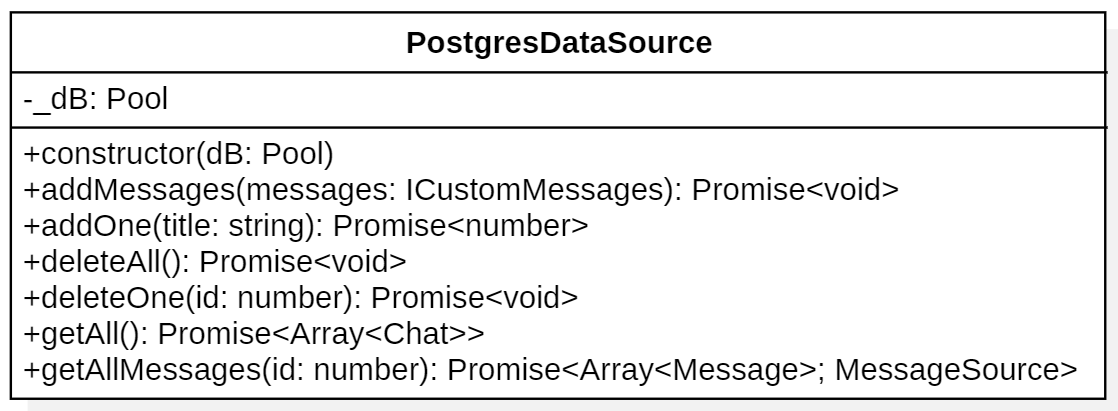
\includegraphics[width=0.6\textwidth]{PostgresDataSource.png}
    \caption{UML della classe PostgresDataSource}
\end{figure}

\subsection{Basi di dati} \label{subsec:basididati}
\subsubsection{ChromaDB}
\textbf{Descrizione}\\
ChromaDB rappresenta il database vettoriale adibito a contenere gli embedding dei documenti caricati nel sistema. Esso contiene due collection di vettori, ovvero una per ogni modello utilizzato nella produzione e consultazione degli embedding.\\
All'interno di ogni collection sono contenuti le informazioni riguardanti gli embedding dei documenti.\\
In particolare, ad ogni oggetto nella collection è associato un valore identificativo ids di tipo \textit{string}, il nome del documento, i metadati ad esso associato e l'effettivo vettore di numeri reali ottenuto dall'embedding del documento.\\ \\
\textbf{Requisiti associati}
\begin{itemize}[itemsep=-4pt]
    \item RFO-27;
    \item RFO-29;
    \item RFD-36;
    \item RFD-37;
    \item RFO-55;
    \item RFO-56;
    \item RFD-57;
    \item RFO-64;
    \item RFO-65;
    \item RIO-4.
\end{itemize}

\subsubsection{MinIO}
\textbf{Descrizione}\\
MinIO rappresenta il database adibito a contenere i documenti caricati nel sistema. Esso contiene due bucket di oggetti rappresentanti i documenti, ovvero uno per ogni modello supportato nell'utilizzo dell'applicazione.\\
All'interno di ogni bucket sono contenuti i documenti, i quali sono rappresentati come oggetti.\\
In particolare, ad ogni oggetto documento nel bucket è associato un nome, una dimensione, la data di inserimento e dei tag. I singoli documenti sono consultabili grazie alla generazione di un link di visualizzazione.\\ \\
\textbf{Requisiti associati}
\begin{itemize}[itemsep=-4pt]
    \item RFO-3;
    \item RFO-4;
    \item RFO-5;
    \item RFO-6;
    \item RFZ-7;
    \item RFO-8;
    \item RFD-9;
    \item RFO-10;
    \item RFO-27;
    \item RFO-29;
    \item RIO-2;
    \item RIO-3.
\end{itemize}

\subsubsection{Postgres}
\textbf{Descrizione}\\
Postgres è il database adibito a contenere le chat history di ogni sessione di conversazione attiva nel sistema.\\
Sono definite due diverse tabelle: la tabella \textit{chat\_threads}, che rappresenta le sessioni di conversazione, e la tabella \textit{messages}, che rappresenta e contiene tutte le informazioni dei singoli messaggi.
\textit{Chat\_threads} è composto da un valore identificativo numerico seriale \textit{id}, da una stringa di testo \textit{title} (il nome della sessione) e da un TIMESTAMP \textit{created\_at}.\\
\textit{Messages} è invece identificata da un \textit{id} VARCHAR e contiene un \textit{thread\_id} che si riferisce all'id di un \textit{chat\_threads}, dal contenuto testuale \textit{content}, dal \textit{role} (chi ha scritto il messaggio), \textit{created\_at}, \textit{sourcePage} (numero di pagina del documento fonte, se il messaggio è una risposta) e \textit{sourceLink} (link del documento fonte, se il messaggio è una risposta).\\ \\
\textbf{Requisiti associati}
\begin{itemize}[itemsep=-4pt]
    \item RFD-48;
    \item RFD-49;
    \item RFD-50;
    \item RFO-52;
    \item RFO-53;
    \item RFO-59;
    \item RFD-60;
    \item RFO-63.
\end{itemize}


\begin{figure}[h!]
    \centering  
    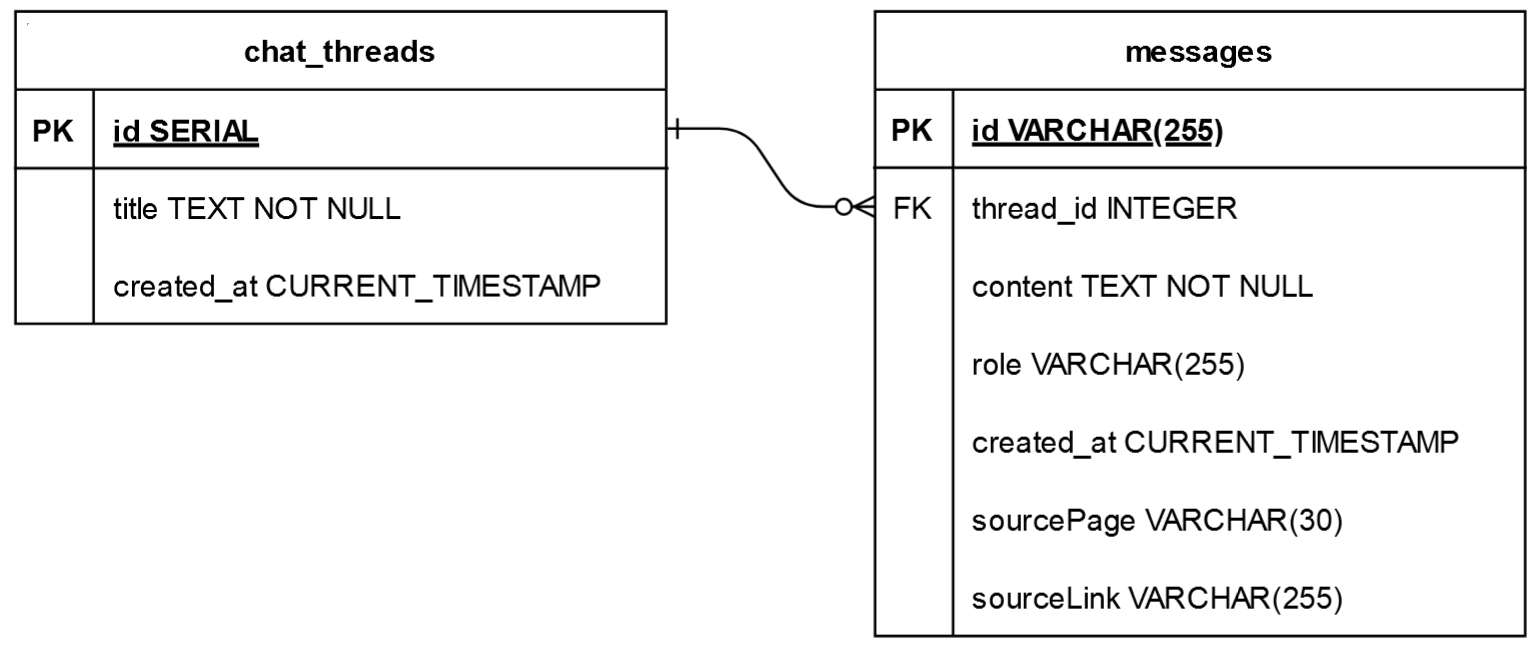
\includegraphics[width=0.8\textwidth]{postgresdb.png}
    \caption{Diagramma ER del database Postgres}
\end{figure}
\vspace{2cm}
\begin{figure}[h!]
    \centering  
    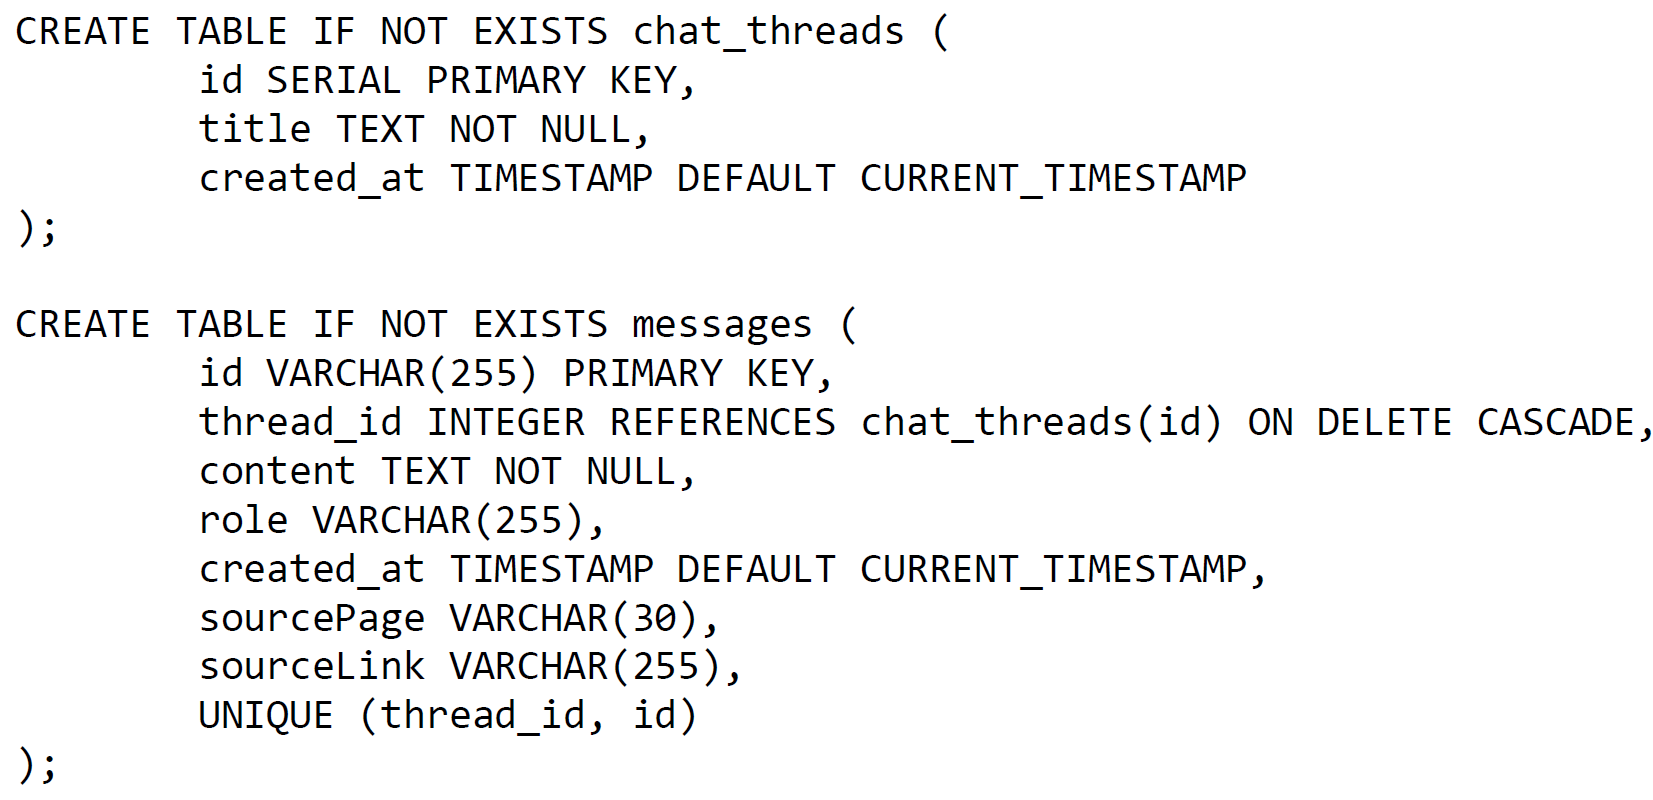
\includegraphics[width=0.8\textwidth]{querypostgresdb.png}
    \caption{Query per la creazione del database Postgres}
\end{figure}

\newpage
